\chapter{Evaluation}\label{chapter:evaluation}

\section{Datasets}

\subsection{IXP Traffic Dataset}

The data used for the evaluation of the system is network traffic collected by GR-IX \cite{gr-ix}. GR-IX is the Greek IXP, through which ISPs exchange traffic between their networks without using their upstream transit providers. GR-IX was founded in 2009 as a successor of AIX (Athens Internet Exchange), which was in operation since 2000. The exchange is managed and operated by the Greek Research and Technology Network (GRNET).

GR-IX is handling aggregate traffic peaking at multiple Gigabytes per second. Using the packet sampling tool sFlow, IP packets were captured with a random sampling rate of 1 out of 2000 over a period of six months (July 2013 to February 2014). During this period of time 1.9 billion packets were captured, which translates to an average of 110 packets sampled per second. The captured packets were preprocessed to extract the following useful fields:
\begin{itemize}
\item \texttt{sourceIP}: source IP address in dot-decimal notation
\item \texttt{destinationIP}: destination IP address in dot-decimal notation
\item \texttt{protocol}: IP protocol number (6 for TCP, 17 for UDP)
\item \texttt{sourcePort}: source port number
\item \texttt{destinationPort}: destination port number
\item \texttt{ipSize}: total length of the IP packet
\item \texttt{dateTime}: Unix timestamp of the packet's capture time
\end{itemize}

\subsection{Autonomous System Dataset}\label{subsection:benchmarks_as_dataset}

One of the external datasets used by the topology is the GeoLite ASN IPv4 database \cite{geolite}. This dataset maps IPv4 address ranges to Autonomous System Numbers (ASN) and is updated by MaxMind every month. The dataset comes in a CSV file, having a size of 13 MB. This file is stored at HDFS in order to be available to the Storm Supervisors. The data contained in it have the following fields:
\begin{itemize}
\item \texttt{ipIntStart}: integer representation of the first IP address contained in the AS
\item \texttt{ipIntEnd}: integer representation of the last IP address contained in the AS
\item \texttt{as}: AS number and name
\end{itemize}

\subsection{DNS Dataset}\label{subsection:benchmarks_dns_dataset}

The other external dataset used by the topology is the Rapid7 Reverse DNS dataset \cite{rdns}. This dataset maps IPv4 addresses to domain names. Rapid7 Labs creates this data by performing a DNS PTR lookup for all IPv4 addresses. It is updated every 2 weeks and is made available at The Internet-Wide Scan Data Repository (scans.io). The data format is a gzip-compressed CSV file, having a size of 5.7 GB compressed and 55 GB uncompressed, while containing 1.2 billion records. The fields of the dataset are:
\begin{itemize}
\item \texttt{ip}: IP address in dot-decimal notation
\item \texttt{dns}: domain name
\end{itemize}

The Reverse DNS dataset is stored in the \texttt{rdns} HBase table. The field \texttt{ip} is used as the row key and \texttt{dns} is stored at a column.


\section{Cluster Description}

To execute the following experiments, we use virtual machines (VMs) operating on the OpenStack cluster hosted by the Computing Systems Laboratory (CSLab) of the School of Electrical and Computer Engineering, NTUA. 

For the performance tuning experiments we create 10 virtual machines:
\begin{itemize}
\item \textbf{Zookeeper:} This is a Zookeeper server in standalone mode, running the QuorumPeerMain application. Zookeeper is providing coordination between the nodes of the Kafka, Storm and HBase clusters.
\item \textbf{Master:} This node is running the master applications for all the clusters. Master runs a Nimbus daemon for Storm, a NameNode and SecondaryNameNode for HDFS and an HMaster for HBase.
\item \textbf{Storm cluster:} The Storm cluster consists of 4 virtual machines running the Supervisor daemon.
\item \textbf{Kafka and HBase cluster:} The Kafka and HBase clusters are co-hosted on 4 virtual machines. Each machine runs a Kafka server, an HDFS DataNode and HRegionServer for HBase. The RegionServer is allowed to have 5 GB of maximum heap size. Kafka CPU usage is very low during all of the benchmarks (around 3\%), therefore co-hosting it with HBase does not interfere with performance.
\end{itemize}

The deployment diagram for the clusters is presented in Figure \ref{figure:benchmarks_cluster_deployment}. Each of the virtual machines has the specifications listed in Table \ref{table:benchmarks_cluster_hw_specs}. The versions of the software used in our experiments are listed in Table \ref{table:benchmarks_cluster_sw_specs}.

To conduct the scalability experiments, we increase the number of nodes in the Storm and Kafka/ HBase clusters up to 16 for each. The rest of the deployment details remain the same.

\begin{figure}[h!]
\centering
\includegraphics[width=\textwidth]{figures/benchmarks_cluster_deployment}
\caption{Cluster deployment diagram}
\label{figure:benchmarks_cluster_deployment}
\end{figure}

\begin{table}[h!]
\centering
\begin{tabular}{ |c|c| }
\hline
Component & Description \\ \hline \hline
CPU & 4 cores @ 2.4 GHz \\ \hline
RAM & 8 GB \\ \hline
Disk & 80 GB \\ \hline
\end{tabular}
\caption{Virtual machine hardware specifications}
\label{table:benchmarks_cluster_hw_specs}
\end{table}

\begin{table}[h!]
\centering
\begin{tabular}{ |c|c| }
\hline
Software & Version \\ \hline \hline
Zookeeper & 3.4.6 \\ \hline
Kafka & 2.10-0.8.2.1 \\ \hline
Storm & 0.9.4 \\ \hline
Hadoop & 2.6.0 \\ \hline
HBase & 1.1.0.1 \\ \hline
Phoenix & 4.4.0-HBase-1.1 \\ \hline
\end{tabular}
\caption{Software versions}
\label{table:benchmarks_cluster_sw_specs}
\end{table}


\section{Kafka Performance and Scalability}

To measure Kafka performance and scalability we use the performance tools ProducerPerformance and TestEndToEndLatency shipped with the Kafka installation. For the following experiments, we set the size of the messages generated by the tools to 62 bytes, to match the average size of the messages produced by real IXP traffic. The topic we use has 4 partitions and a replication factor of 2 for fault tolerance. Replication during the experiments is asynchronous, meaning that the broker acknowledges the write as soon as it has written it to its local log, without waiting for the other replicas to also acknowledge it.

\subsection{Producer Batch Size}\label{subsection:benchmarks_kafka_batch}

The producer can be configured to accumulate data in memory and to send out larger batches in a single request for each partition \cite{kafka_documentation}. \emph{Batching} leads to larger network packets and larger sequential disk operations on the brokers, which allows Kafka to turn a stream of random message writes into linear writes. This increases performance on both the producer and the broker. 

We experiment with different batch sizes and measure the message input throughput for our topic. The effects of batching on throughput can be observed in Table \ref{table:batch_size_throughput} and Figure \ref{figure:benchmarks_kafka_batch_2}.

\begin{table}[h!]
\centering
\begin{tabular}{ |c|c| }
\hline
Batch size & Throughput (messages/sec) \\ \hline \hline
100 & 12658 \\ \hline
200 & 25516 \\ \hline
400 & 49397 \\ \hline
800 & 104597 \\ \hline
1600 & 188730 \\ \hline
3200 & 293877 \\ \hline
6400 & 381859 \\ \hline
\end{tabular}
\caption{Producer batch size effect on topic throughput}
\label{table:batch_size_throughput}
\end{table}

\begin{figure}[h!]
\centering
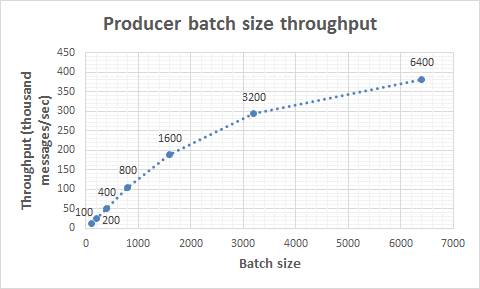
\includegraphics[width=0.8\textwidth]{figures/benchmarks_kafka_batch_2}
\caption{Producer batch size effect on topic throughput}
\label{figure:benchmarks_kafka_batch_2}
\end{figure}

Even though a bigger batch size can increase throughput by orders of magnitude, it also increases the time a message is waits in the producer to be sent in the next batch. Since even a low batch size 100 can achieve greater throughput (12658 messages/sec) than the storm topology in the maximum configuration of our scalability experiment (3988 messages/sec as we will see in Section \ref{section:benchmarks_storm_scalability}), we opt to choose a small batch size in order to reduce message latency. To allow the producer to handle bursts of more packets, we use batch size \textbf{200} for our producer. The rest of the experiments are performed with batch size 200.

\subsection{End-to-End Latency}

Kafka \emph{end-to-end latency} is the time it takes for a message sent by a producer to be delivered to a consumer. For this experiment, the performance tool TestEndToEndLatency creates a producer and a consumer and repeatedly times how long it takes for a producer to send a message to the Kafka cluster and then be received by the consumer. 

The average Kafka end-to-end latency is measured at \textbf{2.871 msec}. Other latency percentiles are presented in Table \ref{table:end-to-end_latency}.

\begin{table}[h!]
\centering
\begin{tabular}{ |c|c| }
\hline
Percentile & Latency (msec) \\ \hline \hline
50th & 2 \\ \hline
99th & 4 \\ \hline
99.9th & 10 \\ \hline
\end{tabular}
\caption{End-to-end latency percentiles}
\label{table:end-to-end_latency}
\end{table}

\subsection{Multiple Producers}

In this experiment we use multiple producers that create messages for a single topic and measure the aggregate message input throughput for the topic. The producers are running on different machines.

Figure \ref{figure:benchmarks_kafka_producers} shows that the aggregate message input throughput increases linearly with the number of the simultaneous producers. This allows us to expand our system to collect and store in Kafka data from multiple different producer sources.

\begin{figure}[h!]
\centering
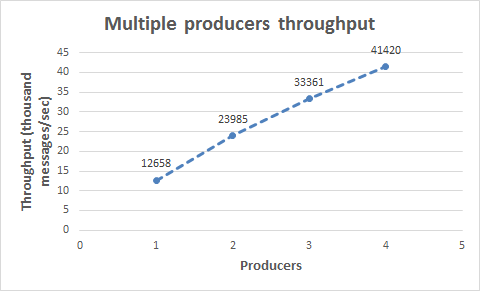
\includegraphics[width=0.8\textwidth]{figures/benchmarks_kafka_producers}
\caption{Topic throughput scalability with the number of producers}
\label{figure:benchmarks_kafka_producers}
\end{figure}

\subsection{Kafka Scalability}

Partitions allow the topic to scale in size by being distributed over the brokers of the cluster and act as the unit of parallelism, providing load balancing over the write and read requests of the producers and the consumers respectively.

To evaluate the scalability of the Kafka topic with the Kafka cluster size, we measure the message input throughput for clusters with different numbers of brokers. The number of the topic's partitions is adjusted according to the number of the brokers.

As we can see in Figure \ref{figure:benchmarks_kafka_scalability} topic throughput scales almost linearly with Kafka cluster size.

\begin{figure}[H]
\centering
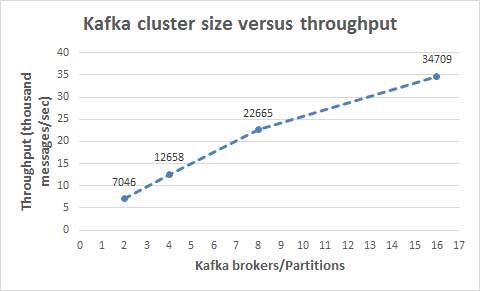
\includegraphics[width=0.8\textwidth]{figures/benchmarks_kafka_scalability}
\caption{Topic throughput scalability with Kafka cluster size}
\label{figure:benchmarks_kafka_scalability}
\end{figure}


\section{Storm Performance Tuning}

The Storm metrics for the following experiments were extracted from the Storm Web UI, which provides information on the running Storm topologies. The CPU metrics were extracted from the Ganglia monitoring system \cite{ganglia} running on the VMs of the evaluation cluster.

\subsection{Parallelism Tuning}\label{subsection:benchmarks_storm_tuning}

To achieve maximum topology throughput, we experiment with the parallelism of its components (spout and bolts). Parallelism tuning in Storm is performed with the help of the capacity metric. 

The \emph{capacity metric} tells us what percentage of the time in the last 10 minutes the bolt spent executing tuples. If this value is close to 1, then the bolt is 'at capacity' and is a bottleneck in our topology. The solution to at-capacity bolts is to increase the parallelism of that bolt. The listing used to compute the capacity metric is:

\begin{lstlisting}[language=C,frame=none]
capacity = (executedTuplesNumber * averageExecuteLatency) / measurementTime
\end{lstlisting}

During the parallelism tuning experiments, when we see that a bolt's capacity is close to 1, we increase its parallelism in the next experiment. We continue tuning until we achieve maximum topology throughput. The parallelism and capacity for each bolt during the parallelism tuning experiments are presented on Table \ref{table:parallelism_tuning}. The name of each experiment denotes the parallelism of each component of the topology: Kafka Spout - Split Fields Bolt - IP to AS Bolt - IP to DNS Bolt - Phoenix Bolt.

Note that capacity is computed based on topology statistics, therefore its value may sometimes appear to be larger than 1. The parallelism of the Kafka Spout is always 4 to match the number of the topic's partitions.

As we can see in Figure \ref{figure:benchmarks_storm_tuning_throughput} we can achieve maximum topology throughput with the parallelism combination \textbf{4-4-4-16-28}. We use these parallelism settings for the rest of the benchmarks.

We also record the average CPU utilization for the Storm and HBase clusters during the tuning experiments and present them in Figure \ref{figure:benchmarks_storm_tuning_cpu}. We notice that the processors of the Storm and HBase clusters are not saturated at maximum topology throughput, which indicates that the topology workload is I/O intensive. This was expected since the IP to DNS Bolt and the Phoenix Blot perform reads and writes respectively to HBase tables.

\begin{table}[h!]
\centering
\resizebox{1\textwidth}{!} {
\begin{tabular}{ |*{9}{c|} }
\hline
\multirow{2}{*}{Experiment} & \multicolumn{2}{|c|}{Split Fields Bolt} & \multicolumn{2}{|c|}{IP to AS Bolt} & \multicolumn{2}{|c|}{IP to DNS Bolt} & \multicolumn{2}{|c|}{Phoenix Bolt} \\ \cline{2-9}
 & Parallelism & Capacity & Parallelism & Capacity & Parallelism & Capacity & Parallelism & Capacity \\ \hline \hline
4-4-4-4-4 & 4 & 0.013 & 4 & 0.011 & 4 & 0.600 & 4 & \textbf{0.987} \\ \hline
4-4-4-12-12 & 4 & 0.021 & 4 & 0.042 & 12 & 0.491 & 12 & \textbf{1.068} \\ \hline
4-4-4-12-20 & 4 & 0.040 & 4 & 0.043 & 12 & \textbf{1.043} & 20 & \textbf{0.911} \\ \hline
4-4-4-16-28 & 4 & 0.043 & 4 & 0.062 & 16 & 0.879 & 28 & \textbf{1.049} \\ \hline
4-4-4-16-36 & 4 & 0.067 & 4 & 0.077 & 16 & 0.816 & 36 & \textbf{1.086} \\ \hline
\end{tabular}
}
\caption{Bolt capacity during parallelism tuning experiments}
\label{table:parallelism_tuning}
\end{table}

\begin{figure}[h!]
\centering
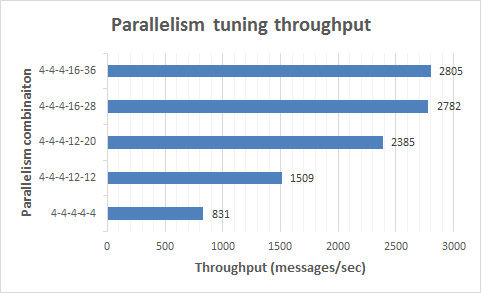
\includegraphics[width=0.8\textwidth]{figures/benchmarks_storm_tuning_throughput}
\caption{Topology throughput during parallelism tuning experiments}
\label{figure:benchmarks_storm_tuning_throughput}
\end{figure}

\begin{figure}[h!]
\centering
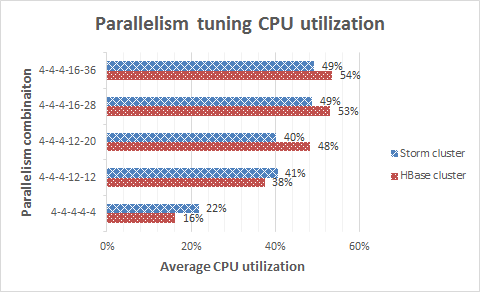
\includegraphics[width=0.8\textwidth]{figures/benchmarks_storm_tuning_cpu}
\caption{Average CPU utilization for the Storm and HBase clusters during parallelism tuning experiments}
\label{figure:benchmarks_storm_tuning_cpu}
\end{figure}

\subsection{Maximum Pending Tuples}

Storm topologies have a \emph{maximum spout pending tuples} parameter. This value puts a limit on the number of tuples that can be in flight (have not yet been acked or failed) in a Storm topology at any point of time. The need for this parameter comes from the fact that Storm uses queues to dispatch tuples from one task to another task. If the consumer side of the queue is unable to keep up with the tuple rate, then the queue starts to build up. Eventually, tuples timeout at the spout and get replayed to the topology, thus adding more pressure on the queues. To avoid this failure case, Storm allows the user to put a limit on the number of tuples that are in flight in the topology. Setting a small maximum pending tuples number can starve the topology from tuples, while a sufficiently large value can overload the topology with a huge number of tuples to the extent of causing failures and replays. 

We experiment with the maximum pending tuples value, while feeding the topology with messages at the maximum rate determined in Subsection \ref{subsection:benchmarks_storm_tuning} (around 2800 messages/sec). The results presented in Table \ref{table:batch_size_throughput} indicate that we can achieve maximum throughput by setting the value of the maximum pending tuples parameter over 100. To allow the topology to handle bursts of more messages, we use the value \textbf{200} for the maximum pending spout tuples parameter. In the case of a message burst, the in-flight tuples will spend more time in the internal queues of the topology, but their number will still be limited by the parameter to avoid failures by overloading.

\begin{table}[h!]
\centering
\begin{tabular}{ |c|c| }
\hline
Maximum pending tuples & Throughput (messages/sec) \\ \hline \hline
10 & 1347 \\ \hline
50 & 2075 \\ \hline
100 & 2782 \\ \hline
200 & 2723 \\ \hline
500 & 2752 \\ \hline
\end{tabular}
\caption{Effect of maximum pending tuples on topology throughput}
\label{table:max_pending_tuples}
\end{table}

\subsection{Bolt Execute Latencies}

A useful metric that allows us to identify the bottlenecks in our topology is the execute latency of each bolt. \emph{Execute latency} is the average time a tuple spends in the execute method of a bolt. 

We record the execute latencies for each bolt of the topology at maximum throughput and present them in Table \ref{table:execute_latencies}. We also compare their relative sizes in Figure \ref{figure:benchmarks_storm_execute_latencies}. It is clear that the tuples spend practically all of their execute time in the IP to DNS Bolt and the Phoenix Bolt. This was expected since these bolts perform reads and writes to HBase tables, while the other bolts execute simple commands in memory.

\begin{table}[h!]
\centering
\begin{tabular}{ |c|c| }
\hline
Bolt & Execute latency (msec) \\ \hline \hline
Split Fields Bolt & 0.047 \\ \hline
IP to AS Bolt & 0.052 \\ \hline
IP to DNS Bolt & 4.779 \\ \hline
Phoenix Bolt & 7.784 \\ \hline
\end{tabular}
\caption{Average execute latency for each bolt of the topology}
\label{table:execute_latencies}
\end{table}

\begin{figure}[H]
\centering
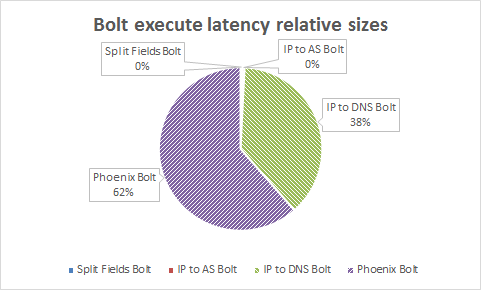
\includegraphics[width=0.8\textwidth]{figures/benchmarks_storm_execute_latencies}
\caption{Relative sizes of execute latencies for the bolts of the topology}
\label{figure:benchmarks_storm_execute_latencies}
\end{figure}

\subsection{Total System Latency}

An important performance indicator for our system is \emph{total system latency}, the time it takes for a message to be sent by the Kafka producer to the topic, consumed by the Kafka Spout, processed by the bolts of the topology and eventually be stored in the Phoenix table and made available for queries.

To compute total system latency we feed the topology with real-time messages and query the table for the row with the latest timestamp. By comparing this timestamp to the current time we can measure the total system latency. Total system latency is measured at \textbf{1.161 sec} on average at maximum topology throughput.

\subsection{Salting Write Performance}\label{subsection:benchmarks_storm_salting}

HBase sequential write suffers from RegionServer hotspotting since the row key is monotonically increasing. Salting the row key provides a way to balance load among the RegionServers, as we described in Section \ref{section:optimizations_salting}.

In this experiment we use a salted and a non-salted table, and compare the throughput of the topology, the write request and CPU utilization on the RegionServers, as well as the execute latency of the Phoenix Bolt. The salted table has 4 salt buckets that are split among the 4 RegionServers of the HBase cluster.

Figures \ref{figure:benchmarks_storm_salting_requests} and \ref{figure:benchmarks_storm_salting_cpu} demonstrate that salting serves its purpose by eliminating write hostspotting. Whereas all the write requests were directed to a single RegionServer for the non-salted table, the load is evenly distributed for the salted table. Note that higher aggregate CPU utilization while using the salted table is linked to better utilization of the cluster's resources, leading to higher topology throughput.

Salting also decreases the Phoenix Bolt's execute latency by \textbf{74\%}, as we can see in Figure \ref{figure:benchmarks_storm_salting_latency}. The execute latency of the Bolt when writing to the non-salted table was increased due to the strain put on the RegionServer that handled all the write requests.

Finally, Figure \ref{figure:benchmarks_storm_salting_throughput} demonstrates that salting massively increases the topology throughput by \textbf{140\%}.

\begin{figure}[H]
\centering
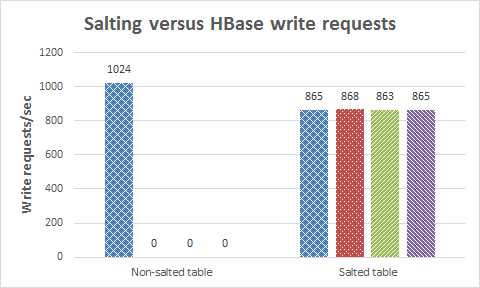
\includegraphics[width=0.8\textwidth]{figures/benchmarks_storm_salting_requests}
\caption{Salting effect on HBase write request distribution}
\label{figure:benchmarks_storm_salting_requests}
\end{figure}

\begin{figure}[H]
\centering
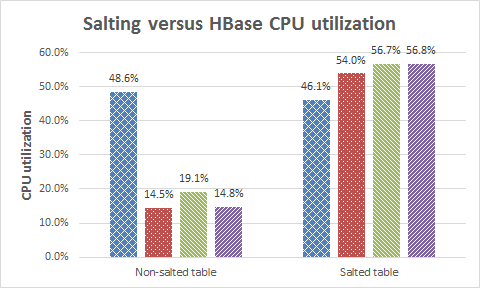
\includegraphics[width=0.8\textwidth]{figures/benchmarks_storm_salting_cpu}
\caption{Salting effect on HBase cluster CPU utilization}
\label{figure:benchmarks_storm_salting_cpu}
\end{figure}

\begin{figure}[H]
\centering
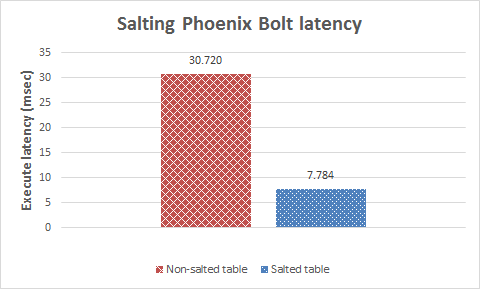
\includegraphics[width=0.8\textwidth]{figures/benchmarks_storm_salting_latency}
\caption{Salting effect on Phoenix bolt latency}
\label{figure:benchmarks_storm_salting_latency}
\end{figure}

\begin{figure}[H]
\centering
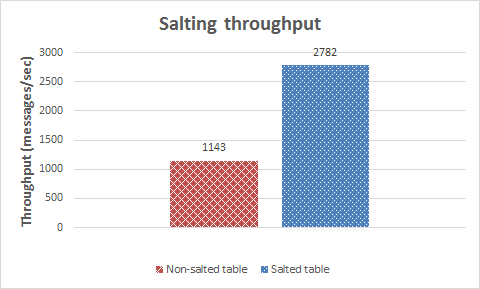
\includegraphics[width=0.8\textwidth]{figures/benchmarks_storm_salting_throughput}
\caption{Salting effect on topology throughput}
\label{figure:benchmarks_storm_salting_throughput}
\end{figure}


\section{Storm Scalability}\label{section:benchmarks_storm_scalability}

To evaluate the scalability of the topology with Storm and HBase cluster size, we measure the topology throughput for different cluster sizes. We increase Storm and HBase cluster sizes simultaneously, meaning that on each test there are as many Supervisors as RegionServers. We also adjust accordingly the number of partitions for the topic, the component parallelism in the topology and the number of salt buckets for the table. After any change to the size HBase cluster we distribute the \texttt{rdns} table evenly among the RegionServers and compact it for data locality.

The topology throughput scalability with Storm and HBase cluster size can be seen in Figure \ref{figure:benchmarks_storm_scalability_throughput}. The average CPU utilization for the Storm and HBase clusters during the scalability experiments is presented in Figure \ref{figure:benchmarks_storm_scalability_cpu}.

\begin{figure}[H]
\centering
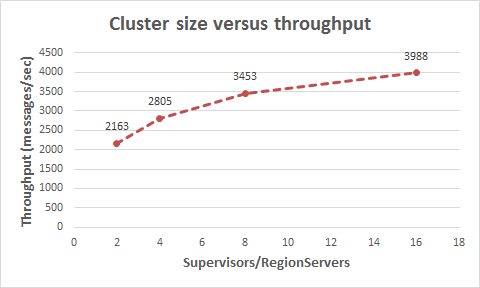
\includegraphics[width=0.8\textwidth]{figures/benchmarks_storm_scalability_throughput}
\caption{Topology throughput scalability with Storm and HBase cluster size}
\label{figure:benchmarks_storm_scalability_throughput}
\end{figure}

\begin{figure}[H]
\centering
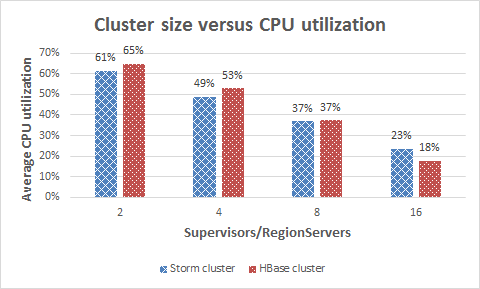
\includegraphics[width=0.8\textwidth]{figures/benchmarks_storm_scalability_cpu}
\caption{Average CPU utilization during scalability experiments}
\label{figure:benchmarks_storm_scalability_cpu}
\end{figure}

We notice that the topology throughput does not scale linearly with Storm and HBase cluster size and the processors are underused for larger cluster sizes. This indicates that the evaluation cluster setup is suffering from disk I/O saturation. As we increase the nodes for each cluster by adding more VMs, the underlying OpenStack cluster infrastructure remains the same, thus the aggregate disk I/O throughput does not increase proportionally with cluster size. This explains the diminishing increases in throughput as we increase the cluster size. If the aggregate disk I/O throughput was increasing according to the cluster size, for example by assigning every node with a dedicated disk, then the topology throughput would then scale linearly with cluster size.


\section{HBase and Phoenix Performance Tuning}

The comparison basis of the following benchmarks is our final Phoenix table, after all optimizations are applied. The table uses Snappy compression and no data block encoding, is split in 3 column families and is salted in 4 buckets. All the tables are compacted and their regions are distributed evenly among the RegionServers. Queries are performed over 10 million rows that are already cached in the BlockCache, unless stated otherwise.

We perform the following two types of queries:

\begin{lstlisting}[language=PhoenixSQL]
SELECT COUNT(*) FROM TABLE netdata;
\end{lstlisting}

The \emph{count} query iterates over the rows of the default column family. This query is useful to measure read performance without any additional calculations.

\begin{lstlisting}[language=PhoenixSQL]
SELECT as.asS, as.asD, COUNT(*) AS pairCount
FROM netdata
GROUP BY as.asS, as.asD
ORDER BY pairCount DESC
LIMIT 10;
\end{lstlisting}

The \emph{topN AS} query returns the top 10 AS pairs in this table ordered by the number of exchanged packets. We also perform the \emph{topN DNS} alternative on some benchmarks, however this query is more computationally intensive, since the \texttt{GROUP BY} clause creates many more distinct pairs for domain names than for autonomous systems. This leads to significantly bigger sets that have to be sorted during the calculations and thus subsequently larger query latency.

\subsection{HDFS Short-Circuit Local Reads}\label{subsection:benchmarks_hbase_short_circuit}

As we described on Section \ref{section:optimizations_short_circuit}, when HDFS short-circuit local reads are enabled, the RegionServer reads local data directly from the disk instead of going through the DataNode. This speeds up data transfer from the disk to the BlockCache when the data is local.

In this experiment we perform a count query over 1 million rows, at first with HDFS short-circuit local reads disabled and afterwards enabled. We measure the total query latency, which includes data transfer time to the BlockCache as well as query processing time. 

When HDFS short-circuit local reads are enabled total query time is reduced by \textbf{62\%}, as we can see in Figure \ref{figure:benchmarks_hbase_short_circuit_latency}.

\begin{figure}[H]
\centering
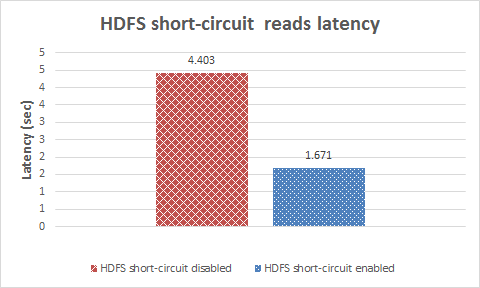
\includegraphics[width=0.8\textwidth]{figures/benchmarks_hbase_short_circuit_latency}
\caption{Enabling HDFS short-circuit for local reads effect on count query latency}
\label{figure:benchmarks_hbase_short_circuit_latency}
\end{figure}

\subsection{Compression and Data Block Encoding}\label{subsection:benchmarks_compression_encoding}

Compression and data block encoding can be used to reduce on-disk data size as well as in-cache data size, as we described in Section \ref{section:compression_encoding}. However this comes with a performance hit for decompression, decoding or both when reading the cached data.

In our experiment we compare on-disk size and in-cache query latency for the following tables:
\begin{itemize}
\item The first table has Fast Diff encoding enabled for all of its column families.
\item The second table has Snappy compression enabled for all of its column families. Compressed BlockCache is enabled.
\item The last table has both Fast Diff encoding enabled and Snappy compression enabled for all of its column families. Compressed BlockCache is enabled.
\end{itemize}

As we can see in Figure \ref{figure:benchmarks_hbase_compression_encoding_size}, using both compression and data block encoding reduces the data size further than the other options. Reduced data size allows more rows can me cached at the same time and reduces data transfer time from the disk to the BlockCache.

However, the best in-cache query latency is achieved by compression alone, as seen in Figure \ref{figure:benchmarks_hbase_compression_encoding_latency}. The data size difference between the second and the third tables is not big enough to outweigh the query latency advantage of the compressed table. This is the reason why we chose compression and no data block encoding for our final table.

\bigskip
\bigskip
\bigskip

\begin{figure}[H]
\centering
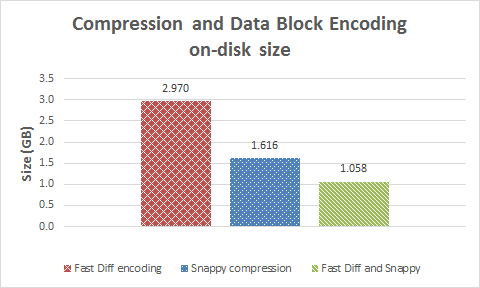
\includegraphics[width=0.8\textwidth]{figures/benchmarks_hbase_compression_encoding_size}
\caption{Compression and data block encoding effect on the on-disk size of a 10 million row table}
\label{figure:benchmarks_hbase_compression_encoding_size}
\end{figure}

\begin{figure}[H]
\centering
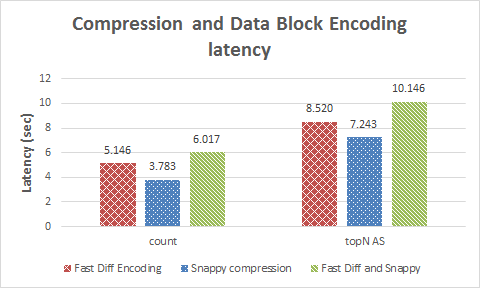
\includegraphics[width=0.8\textwidth]{figures/benchmarks_hbase_compression_encoding_latency}
\caption{Compression and data block encoding effect on query latency}
\label{figure:benchmarks_hbase_compression_encoding_latency}
\end{figure}

\subsection{Number of Column Families}

We compare query performance between our final table, that includes three column families (d, as, dns), and the table containing the same data in one column family. Data is cached by column family, which means that count queries only cache the default family and topN AS queries cache only the as family.

The total size of the final table is divided between the three column families, with the percentages shown in Figure \ref{figure:benchmarks_hbase_cf_sizes}. We measure the total query latency, including data transfer time to the BlockCache, for queries over 1 million rows on the aforementioned tables and present the performance boost that multiple column families offer in Figure \ref{figure:benchmarks_hbase_cf_total_latency}.

\begin{figure}[H]
\centering
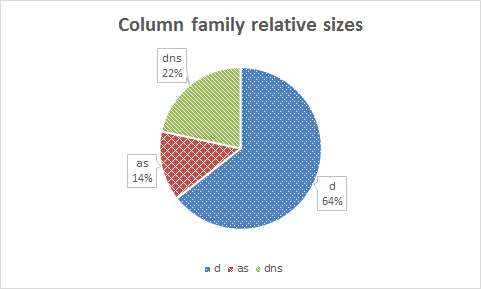
\includegraphics[width=0.8\textwidth]{figures/benchmarks_hbase_cf_sizes}
\caption{Relative sizes of the three column families of the table}
\label{figure:benchmarks_hbase_cf_sizes}
\end{figure}

\begin{figure}[H]
\centering
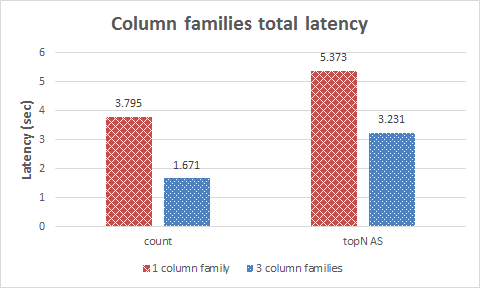
\includegraphics[width=0.8\textwidth]{figures/benchmarks_hbase_cf_total_latency}
\caption{Total query latency for tables with different column family setups}
\label{figure:benchmarks_hbase_cf_total_latency}
\end{figure}

\bigskip

\subsection{Salting Read Performance}\label{subsection:benchmarks_hbase_salting}

As we mentioned in Section \ref{section:optimizations_salting}, aside from write throughput salting can also improve read throughput. Phoenix scans the salted data, sorted within each bucket, in parallel and merge-sorts them at the Phoenix client.

In this experiment we perform a count and a topN AS query on a non-salted and a salted table and compare the query latency. Salting speeds up count and topN AS queries by \textbf{68\%}, as we can see in Figure \ref{figure:benchmarks_hbase_salting_latency}.

\begin{figure}[H]
\centering
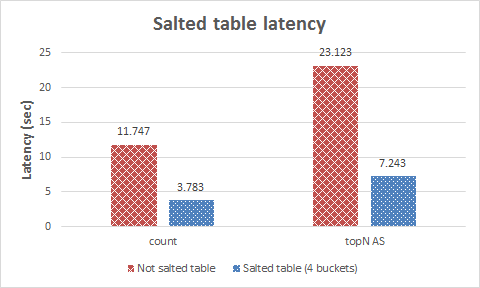
\includegraphics[width=0.8\textwidth]{figures/benchmarks_hbase_salting_latency}
\caption{Salting effect on query latency}
\label{figure:benchmarks_hbase_salting_latency}
\end{figure}


\section{HBase and Phoenix Scalability}

\subsection{Table Rows}

To evaluate the query latency scalability of our table with the size of the data included in the table, we measure the query latency for tables with different numbers of rows. Figures \ref{figure:benchmarks_hbase_rows_latency_1} and \ref{figure:benchmarks_hbase_rows_latency_2} show that the query latency scalability with the size of the data is close to linear.

\begin{figure}[H]
\centering
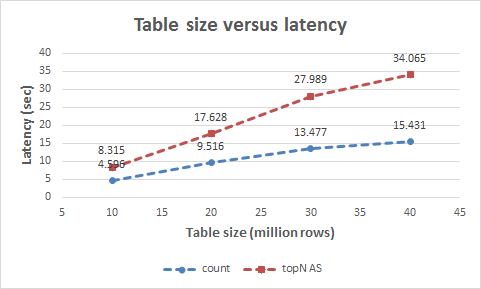
\includegraphics[width=0.8\textwidth]{figures/benchmarks_hbase_rows_latency_1}
\caption{Count and topN AS query latency scalability with table size}
\label{figure:benchmarks_hbase_rows_latency_1}
\end{figure}

\begin{figure}[H]
\centering
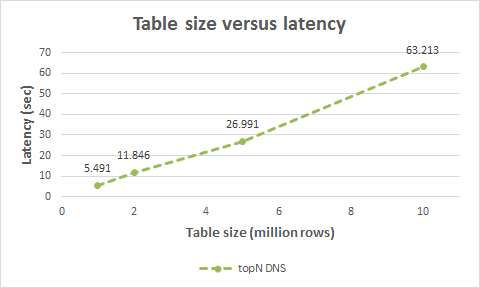
\includegraphics[width=0.8\textwidth]{figures/benchmarks_hbase_rows_latency_2}
\caption{TopN DNS query latency scalability with table size}
\label{figure:benchmarks_hbase_rows_latency_2}
\end{figure}

\subsection{HBase Cluster Size}

To evaluate the scalability of our table with the HBase cluster size, we measure the query latency for clusters with different numbers of RegionServers. The number of the table's salt buckets is adjusted according to the number of the RegionServers. The results of this experiment are presented in Figure \ref{figure:benchmarks_hbase_scalability_latency}.

\begin{figure}[H]
\centering
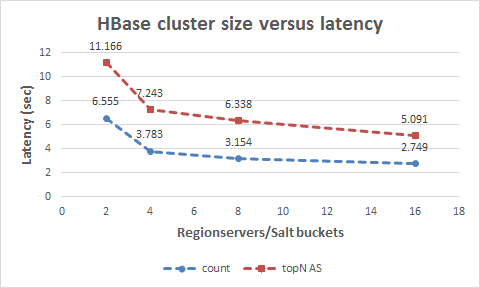
\includegraphics[width=0.8\textwidth]{figures/benchmarks_hbase_scalability_latency}
\caption{Query latency scalability with HBase cluster size}
\label{figure:benchmarks_hbase_scalability_latency}
\end{figure}

\subsection{Multiple Simultaneous Queries}

In this experiment we perform simultaneously the same query from multiple Phoenix clients and measure the average query latency. The clients are running on different machines. 

Figure \ref{figure:benchmarks_hbase_phoenix_clients} shows that multiple queries performed at the same time from different have an additive impact on the average query latency. Since reducing query latency is our priority, multiple simultaneous queries should be avoided.

\begin{figure}[H]
\centering
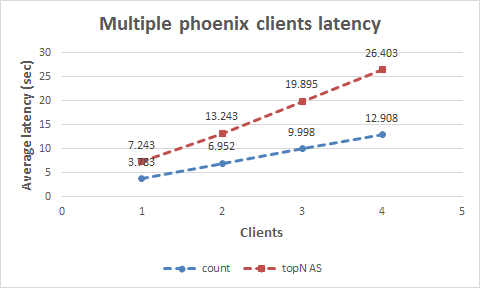
\includegraphics[width=0.8\textwidth]{figures/benchmarks_hbase_phoenix_clients}
\caption{Query latency scalability with the number of Phoenix clients}
\label{figure:benchmarks_hbase_phoenix_clients}
\end{figure}


\cleardoublepage
